% By zmienic jezyk na angielski/polski, dodaj opcje do klasy english lub polish
\documentclass[polish, 12pt]{aghthesis}
\usepackage{babel}
\usepackage[utf8]{inputenc}
\usepackage{url}
\usepackage{indentfirst}

\author{Dawid Romanowski, Wojciech Czarny}

\title{Implementacja metody SPH \\ na procesory graficzne}

\supervisor{dr hab.\ inż.\ Krzysztof Boryczko, prof.\ nadzw.\ AGH}

\date{2014}

% Szablon przystosowany jest do druku dwustronnego, 
\begin{document}

\maketitle{}

\tableofcontents
\clearpage



\section{Opis problemu}

	Symulacja czasu rzeczywistego zjawisk fizycznych jest zagadnieniem złożonym zarówno od strony teoretycznej, jak i od strony implementacyjnej. Aby uzyskać realistycznie wyglądający efekt wymagane jest opracowanie szczegółowego modelu fizycznego danego zjawiska, zapisanie go w taki sposób aby umożliwić jego implementację i na końcu olbrzymia moc obliczeniowa, aby móc podziwiać efekty działania modelu w czasie rzeczywistym. Pierwsze dwa kroki są zależne od nas i możemy je do woli szlifować, jednak w obliczu zbyt małej mocy procesorów jedyny możliwy efekt końcowy do zbiór danych wyjściowych otrzymywany po wykonaniu wszystkich obliczeń - rzecz bezużyteczna w symulacjach czasu rzeczywistego takich jak na przykład gry komputerowe.
	
	$\,$

	W symulacji zjawisk fizycznych często występuje konieczność wykonywania dużej ilość prostych, powtarzalnych obliczeń dla różnych elementów układu. Przykładem może być symulacja zachowania źdźbeł trawy w szerokim polu. Mogą być ich miliony, a dla każdego z nich musimy wykonać podobne obliczenia zależne od takich czynników jak: kierunek wiatru, nacisk otaczających elementów czy ukształtowanie podłoża. CPU nie będzie w stanie nadążyć przy tak olbrzymiej liczbie elementów, nawet jeśli odpowiednio wykorzystamy wszystkie dostępne rdzenie. 
	
	$\,$

		Gdy procesory przestały znacząco zwiększać swoją prędkość taktowania, a zaczęła rosnąć ich koegzystentna ilość, popularniejsze stało się przeprowadzanie niezależnych, zrównoleglonych obliczeń w celu pełnego wykorzystania potencjału sprzętu. GPGPU (general purpose computation on graphics processing unit) to technika wykonywania równoległych obliczeń na procesorach graficznych, która zyskuje na popularności w ostatnich latach. Wynika to z tego, że w nowoczesnych GPU wykorzystywany jest model obliczeniowy SIMT (single instruction, multiple threads), który w połączeniu z ogromną (w stosunku do CPU) ilością rdzeni (setki, czy nawet tysiące) sprawia, że implementacje pewnych algorytmów mogą uzyskać olbrzymie przyspieszenie.
		
	$\,$

	Przedmiotem naszych zainteresowań jest efektywna symulacja zachowania cieczy newtonowskiej, co może być wykorzystane np. w grach wideo. Do sprawdzenia poprawności wykonywanej symulacji służy nam benchmark o nazwie "przerwanie tamy". Polega on na początkowym umiejscowieniu cząstek w pozycji podobnej do przedstawionej na rysunku (\ref{przerwanie_tamy}), a następnie rozpoczęciu symulacji. 
	
	\begin{figure}[h!]
	\centering
		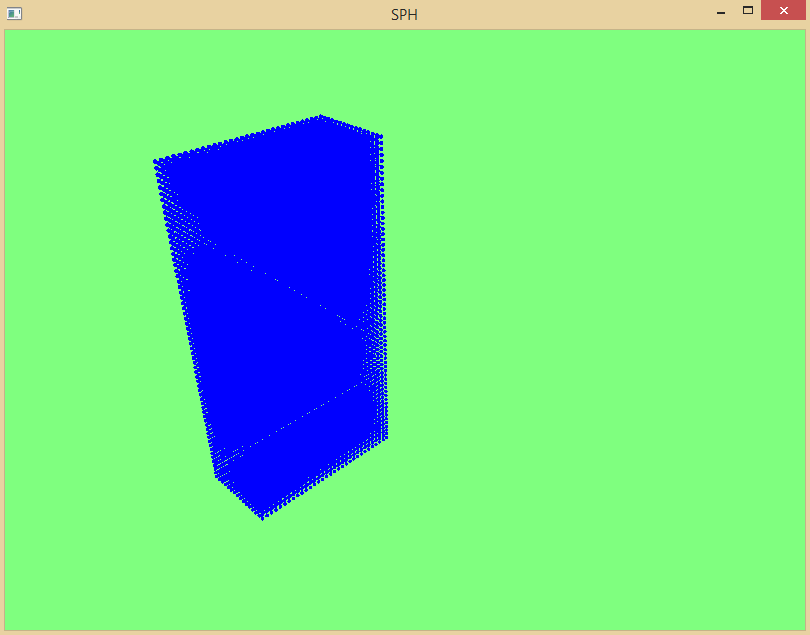
\includegraphics[width=0.8\textwidth]{starting_position.png}
		\caption{Przykładowa pozycja początkowa benchmarku "przerwanie tamy"}
		\label{img:przerwanie_tamy}
	\end{figure}
	
	W przypadku symulacji zachowania płynów nie jest możliwa wizualizacja wyników w czasie wykonywania obliczeń, gdy obliczenia uwzględniają wszystkie oddziaływania pomiędzy elementami modelu fizycznego. Konieczna jest zatem dyskretyzacja problemu oraz przyjęcie uproszczonych zjawisk lub zastąpienie ich prostszymi rozwiązaniami aproksymującymi ich zachowania. Istnieje wiele metod symulowania cieczy - DPD (dissipative particle dynamics), SPH (smoothed particle hydrodynamics) czy SDPD (smoothed dissipative particle dynamics), każda mająca swoje zalety i wady.
	
	$\,$

	Zadaniem naszej pracy jest implementacja metody SPH w technice GPGPU oraz stworzenie aplikacji, która umożliwi wizualizację zachowania cieczy w trakcie wykonywania benchmarku "przerwanie tamy". Pomimo iż metoda ta została pierwszy raz zaproponowana w roku 1977, to dopiero od niedawna możliwe jest jej wykorzystanie do zaprezentowania wyników w czasie rzeczywistym.


\section{Zakres funkcjonalności}

	Nasz projekt to aplikacja wykorzystująca przede wszystkim technologie OpenCL i OpenGL, w której można wyróżnić front-end (tj. wizualizację wykonaną przy pomocy OpenGL) oraz back-end (obliczenia, które symulują zachowanie cieczy). Jako, że obie wymienione technologie wykorzystują procesory graficzne, komunikacja między back-endem a front-endem została zrealizowana poprzez współdzielone bufory na karcie graficznej. 

	Aplikacja umożliwia poruszanie się po wirtualnym świecie przy pomocy klawiszy WSAD oraz lewego przycisku myszy, restartowanie symulacji przy pomocy prawego przycisku myszy oraz dobieranie parametrów symulacji takich jak lepkość czy gęstość cieczy etc.

\section{Wybrane aspekty realizacji}

	\begin{itemize}
		\item Do stworzenia okna i obsługi interakcji użytkownika z aplikacją posłużyła nam biblioteka GLFW.
		\item Skonstruowany został prosty framework, który umożliwił nam przyjemne mapowanie interakcji użytkownika na zachowania wewnątrz aplikacji. Pomogła nam w tym biblioteka Boost a w szczególności Boost.Signals2 umożliwiająca implementacją systemu zdarzeń.
		\item Do renderowania wykorzystaliśmy bibliotekę OpenGL. Kluczowa w osiągnięciu dobrych wyników okazał się dobór odpowiedniej techniki rysowania sfer zwanej “impostor sphere”.
		\item Do GPGPU wykorzystaliśmy bibliotekę OpenCL. Zdecydowaliśmy się korzystać z API w języku C a nie C++ ze względu na lepszą dokumentację.
		\item Konieczna była komunikacja między OpenGL i OpenCL. Wykorzystaliśmy do tego część OpenCL zwaną OpenCL/OpenGL interop.
		\item Całość projektu była zarządzana przy pomocy CMake. Wykorzystaliśmy tylko wieloplatformowe otwarte biblioteki co sprawia, że nasza aplikacja działa zarówno na systemach Linux jak i Windows.
	\end{itemize}
	
\section{Sposób testowania tworzonego oprogramowania}

	Przeprowadzana symulacja w dużej mierze była czymś dla nas nieprzewidywalnym. Nie byliśmy w stanie obliczyć przykładowych poprawnych rozwiązań metody SPH, które później wykorzystalibyśmy do testów jednostkowych, ponieważ najmniejsza zmiana w metodzie mogła całkowicie zaburzyć wyniki. Część systemu odpowiedzialna za grafikę także mogła być testowana tylko naocznie. Postanowiliśmy więc porzucić pomysł stosowania testów automatycznych, ze względu na brak oczywistego i użytecznego sposobu na wdrożenie ich w kluczowych miejscach wytwarzanego przez nas systemu.
	 
	 Stosowane przez nas techniki testowania naszego systemu polegały w dużej mierze na tworzeniu przejrzystych i precyzyjnych logów aplikacji oraz na naocznym sprawdzaniu rezultatów działania symulacji. 
	 
	 Logi okazały się szczególnie przydatne kiedy implementowaliśmy samą metodę SPH w OpenCL. Zapisywaliśmy do nich wyniki kompilacji jąder OpenCL, dzięki czemu ominęliśmy wiele godzin szukania drobnych błędów składniowych w tychże jądrach. 
	 
	 Naoczne sprawdzanie rezultatów działania aplikacji było jedyną możliwą opcją w kwestii potwierdzenia poprawności zaimplementowanej metody ponieważ głównym testem naszej aplikacji było to, czy uzyskany rezultat przypomina w swoim zachowaniu rzeczywistą ciecz. Zachowanie się cząstek w sposób przypominający ciecz jest rzeczą na tyle złożoną, że uzyskanie takiego efektu w dużej mierze potwierdza poprawność zaimplementowanych algorytmów. 
	 

\section{Organizacja pracy}

	Pierwsze rozmowy z klientem składały się głównie z omawiania tematu pracy, tłumaczenia modeli fizycznych oraz omawiania sposobu implementacji. 

	W związku z tym, że GPGPU było dla nas czymś nowym pierwsze tygodnie poświęciliśmy na naukę technologii OpenCL oraz na doszlifowanie wiedzy o OpenGL. Dalsze prace podzieliliśmy na trzy iteracje.

	Pierwszą iteracją było stworzenie aplikacji okienkowej, która umożliwiała wyświetlanie przebiegu symulacji oraz stworzenie atrapy symulacji w OpenCL, ponieważ bez tego nie mieliśmy możliwości weryfikowania uzyskanych wyników.

	W drugiej iteracji zaimplementowaliśmy algorytm SPH korzystając z OpenCL. Wynikiem drugiej iteracji była prawie w całości działająca aplikacja, niemniej jednak były pewne błędy, zarówno implementacyjne jak i wynikające z przyjętego modelu, które musiały zostać wyeliminowane.

	Trzecia iteracja to poprawki w modelu obliczeń, debugowanie kodu oraz dodatki umożliwiające łatwiejszą interakcją użytkownika z aplikacją oraz redagowanie dokumentacji.

	Wizualizacja została napisana przez Dawid Romanowskiego, natomiast symulacja została w większości napisana przez Wojciecha Czarnego. Ze względu na poziom skomplikowania algorytmu SPH w trakcie implementacji symulacji korzystaliśmy z technik pair programming i rubber duck debugging.

	W ostatniej iteracji Wojciech Czarny zajmował się naprawianiem usterek i testowaniem, natomiast Dawid Romanowski redagowaniem dokumentacji z zebranych w trakcie prac notatek.

\section{Wyniki projektu}

	W wyniku pracy nad projektem powstały:
	\begin{itemize}
	\item aplikacja do symulowania zachowania cieczy metodą SPH
	\item dokumentacja składająca się z dokumentacji procesowej, technicznej i użytkownika.
	\end{itemize}

	\bibliography{bibliografia}

\end{document}
